\section{Trade-offs}
\subsection{Circuit overhead}
Let $p$ be the probability that Tor Browser submits an SFO to a sampled CTR on a
fresh independent circuit, and $\mathcal{D}$ a distribution that describes how
many SFOs are presented on a website visit.  As shown in
Equation~\ref{eq:sub-oh}, we can now estimate the resulting circuit overhead.
\begin{equation} \label{eq:sub-oh}
	f(p,\mathcal{D}) =
		\frac{p}{n} \sum_{i=1}^{n} c_i, \textrm{where } c_i\sample\mathcal{D}
\end{equation}

We decided to approximate $\mathcal{D}$ using the $n$ most popular webpages
submitted to Reddit (r/frontpage, all time) as of December 4, 2019.\footnote{%
	\url{https://github.com/pylls/padding-machines-for-tor/commit/353bfa75e9f7d6aa0a1dff9516ff234cbf0f4562}
} This was motivated by the intuition that such webpages should include more
resources than basic frontpages, such that $\mathcal{D}$ is more likely to be
overestimated rather than underestimated.  This should further be the case
because we collected the SFO data set using fresh Chromium instances, simply
harvesting all SFOs that appeared in NetLog.  In other words, due to some
initial call-home behavior on start-up, a few additional SFOs are included per
data point.

Using $p=\frac{1}{10}$ and plugging our approximated $\mathcal{D}$ into
Equation~\ref{eq:sub-oh}, the resulting circuit overhead is $0.70$.  It should be
noted that these circuits are \emph{light} in terms of bandwidth when compared
to loading an entire website.

\begin{figure}
	\centering
	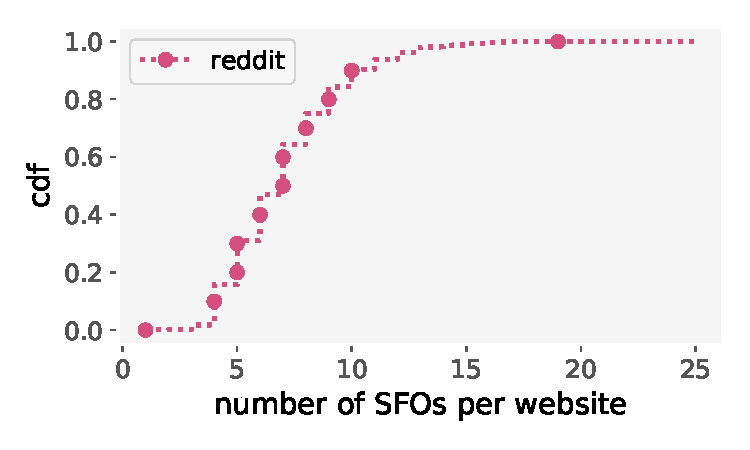
\includegraphics[width=\columnwidth]{../exp/plot/img/sfo-dist}
	\caption{%
		SFO distribution derived from the most frequently viewed reddit pages as
		of December 4, 2019.
	}
	\label{fig:sfo-dist}
\end{figure}

\subsection{SFO Timeouts}
Large timeouts imply less chance that an SFO is leaked to more parties
unnecessarily (privacy).  Small timeouts reduce the attacker's window to
intervene (security).

\subsubsection{Tor Browser}
Recommend a value based on transmitting \texttt{ct-max-sfo-bytes} over many
independent circuits, which gives us a distribution that can be considered.

\subsubsection{CTR}
Recommend a value based on fetching inclusion proofs from several different
logs over Tor, which gives us a distribution that can be considered.  Use the
results from Tor Browser and CTR to reason about \texttt{ct-report-timeout}.
